\chapter{Tutorial: Processing Mars Orbiter Camera Imagery}
\label{ch:tutorial}

\definecolor{lgray}{gray}{0.95}

\section{Quick Start}

The Stereo Pipeline package contains command-line programs that
convert a stereo pair in ISIS {\em cube} format into a 3D ``point
cloud'' image: \texttt{\textit{stereo-output}-PC.tif}.  This is an
intermediate format that can be passed along to one of several
programs that convert a point cloud into a mesh for 3D viewing or a
gridded digital elevation model (DEM) for GIS purposes.

There are a number of ways to fine-tune parameters and analyze the
results, but ultimately this software suite takes images and builds
models in a mostly automatic way.  To create a point cloud file, you
simply pass two image files to the \texttt{stereo} command:

\hspace*{2em}\texttt{ISIS 3> stereo \textit{image\_file1 image\_file2 stereo-output}}
\smallskip

You can then make a mesh or a \ac{DEM} file with the following
commands (the \texttt{\textit{stereo-output}-PC.tif} and
\texttt{\textit{stereo-output}-L.tif} files are created by the
\texttt{stereo} program above):

\hspace*{2em}\texttt{ISIS 3> point2mesh \textit{stereo-output}-PC.tif \textit{stereo-output}-L.tif}
\smallskip

\hspace*{2em}\texttt{ISIS 3> point2dem \textit{stereo-output}-PC.tif \textit{stereo-output}-L.tif}
\smallskip

All files output by Stereo Pipeline will start with the same prefix,
which above was set to \texttt{\textit{stereo-output}}. If it is desired
that the outputs go to a subdirectory, specify it as part of the
prefix. For example, using \texttt{\textit{results/run}} for the output
prefix, will ensure that all files are in the \texttt{\textit{results/}} directory.

\section{Preparing the Data}

The data set that is used in the tutorial and examples below is a
pair of Mars Orbital Camera (\ac{MOC}) \citep{1992JGR....97.7699M,2001JGR...10623429M}
images whose \ac{PDS} Product IDs are M01/00115 and E02/01461.
This data can be downloaded from the PDS directly, or they can be
found in the \texttt{data/MOC/} directory of your Stereo Pipeline distribution.

\subsection{Loading and Calibrating Images using ISIS}

These raw \ac{PDS} images (\texttt{M0100115.imq} and \texttt{E0201461.imq})
need to be imported into the \ac{ISIS} environment and radiometrically
calibrated.  You will need to be in an \ac{ISIS} environment (have
set the \texttt{ISISROOT} environment variable and sourced the
appropriate \ac{ISIS} 3 Startup script, as detailed in the \ac{ISIS}
3 instructions; we will denote this state with the `\texttt{ISIS
3>}' prompt).  Then you can use the \texttt{mocproc} program, as follows:

\begin{verbatim}
    ISIS 3> mocproc from= M0100115.imq to= M0100115.cub Mapping= NO
    ISIS 3> mocproc from= E0201461.imq to= E0201461.cub Mapping= NO
\end{verbatim}

There are also \texttt{Ingestion} and \texttt{Calibration} parameters
whose defaults are `\texttt{YES}' which will bring the image into the
\ac{ISIS} format and perform radiometric calibration.  By setting the
\texttt{Mapping} parameter to `\texttt{NO}' the resultant file will be
an \ac{ISIS} cube file that is calibrated, but not map-projected.
Note that while we have not explicitly run \texttt{spiceinit}, the
Ingestion portion of \texttt{mocproc} quietly ran \texttt{spiceinit}
for you (you'll find the record of it in the \ac{ISIS} Session Log,
usually written out to a file named \texttt{print.prt}).  Refer to
Figure~\ref{p19-images} to see the results at this stage of
processing.

\begin{figure}[t!]
\begin{minipage}{5.2in}
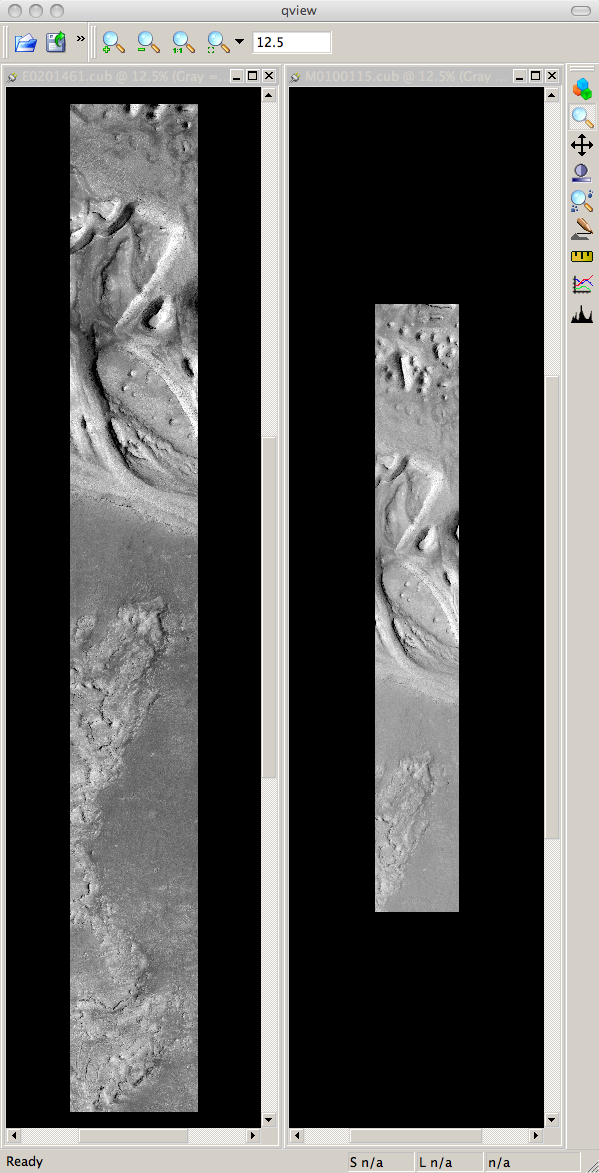
\includegraphics[height=3.7in]{images/p19-images.png}
\hfill
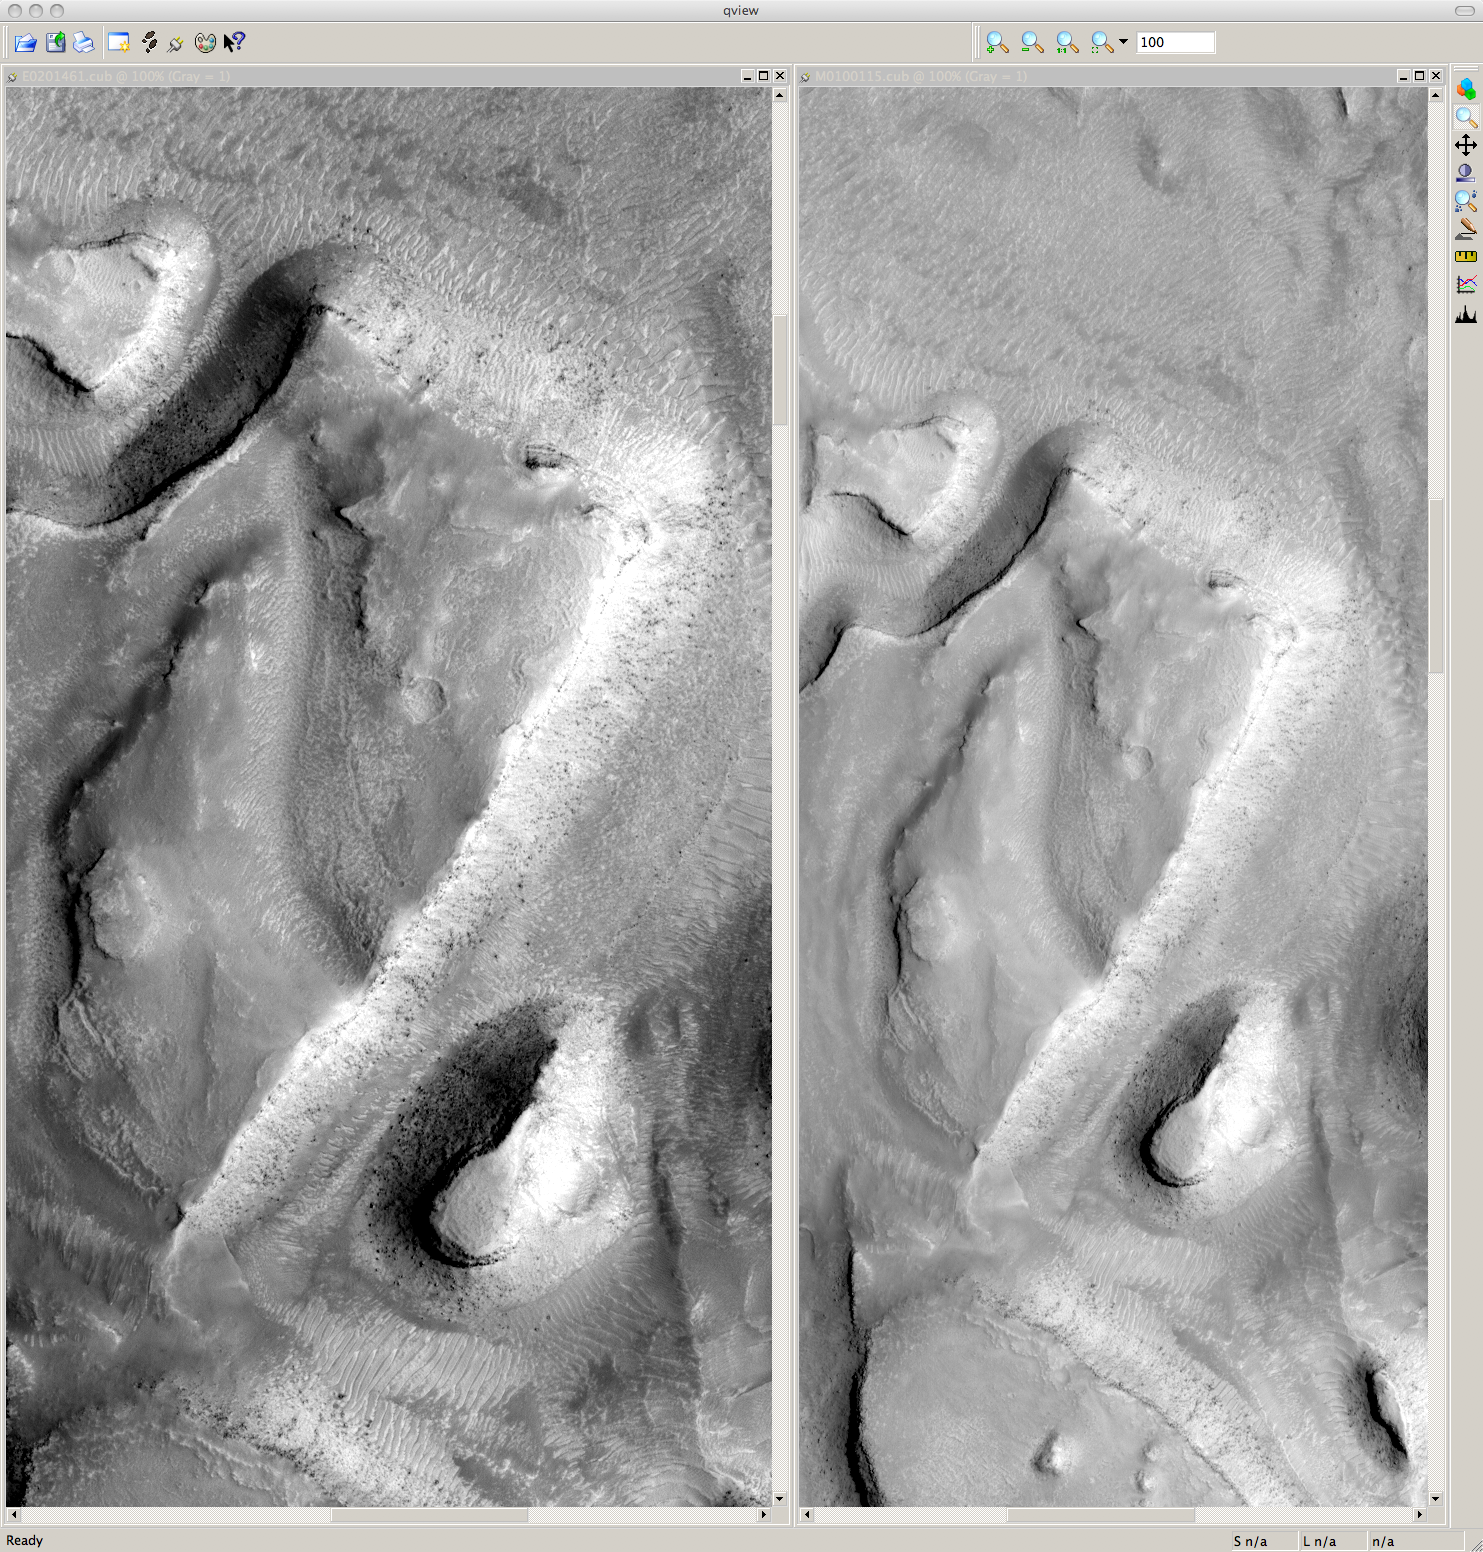
\includegraphics[height=3.7in]{images/p19-images_zoom.png}
\end{minipage}
\hfill
\begin{minipage}{1.3in}
\caption[P19 images open in qview zoomed in]{
    \label{p19-images}
    This figure shows \texttt{E0201461.cub} and \texttt{M0100115.cub}
    open in ISIS's qview program.  The view on the left shows their
    full extents at the same zoom level, showing how they have
    different ground scales.  The view on the right shows both images
    zoomed in on the same feature.  }
\end{minipage}
\end{figure}

\subsection{Aligning Images}
\label{sec:AligningImages}

The images also need to be rectified (or aligned).  There are many
ways to do this (see using \texttt{alignment-method} in \texttt{stereo}'s
\texttt{stereo.default} file in section
\ref{settingoptionsinstereodefault}).  The most straightforward
process is to align the images by map-projecting them in \ac{ISIS}.
This example continues with the files from above, \texttt{E0201461.cub}
and \texttt{M010015.cub}.

This section describes the theory behind doing each of these steps,
but we also provide the \texttt{cam2map4stereo.py} program (page
\pageref{cam2map4stereo}) which performs these steps automatically
for you.

The \ac{ISIS} \texttt{cam2map} program will map-project these images:

\begin{verbatim}
  ISIS 3> cam2map from=M0100115.cub to=M0100115.map.cub
  ISIS 3> cam2map from=E0201461.cub to=E0201461.map.cub map=M0100115.map.cub matchmap=true
\end{verbatim}

Notice the order in which the images were run through
\texttt{cam2map}. The first projection with \texttt{M0100115.cub}
produced a map-projected image centered on the center of that image.
The projection of \texttt{E0201461.cub} used the \texttt{map=}
parameter to indicate that \texttt{cam2map} should use the same map
projection parameters as those of \texttt{M0100115.map.cub} (including
center of projection, map extents, map scale, etc.) in creating the
projected image. By map-projecting the image with the worse resolution
first, and then matching to that, we ensure two things: (1) that the
second image is summed or scaled down instead of being magnified up,
and (2) that we are minimizing the file sizes to make processing in
the Stereo Pipeline more efficient.

Technically, the same end result could be achieved by using the
\texttt{mocproc} program alone, and using its \texttt{map=
M0100115.map.cub} option for the run of \texttt{mocproc} on
\texttt{E0201461.cub} (it behaves identically to \texttt{cam2map}).
However, this would not allow for determining which of the two
images had the worse resolution and extracting their minimum
intersecting bounding box (see below).  Furthermore, if you choose
to conduct bundle adjustment (see Chapter \ref{ch:bundle_adjustment},
page \pageref{ch:bundle_adjustment}) as a pre-processing step, you
would do so between \texttt{mocproc} (as run above) and \texttt{cam2map}.

The above procedure is in the case of two images which cover similar
real estate on the ground.  If you have a pair of images where one
image has a footprint on the ground that is much larger than the
other, only the area that is common to both (the intersection of their
areas) should be kept to perform correlation (since non-overlapping
regions don't contribute to the stereo solution).  If the image with
the larger footprint size also happens to be the image with the better
resolution (i.e. the image run through \texttt{cam2map} second with
the \texttt{map=} parameter), then the above \texttt{cam2map}
procedure with \texttt{matchmap=true} will take care of it just fine.
Otherwise you'll need to figure out the latitude and longitude
boundaries of the intersection boundary (with the \ac{ISIS}
\texttt{camrange} program).  Then use that smaller boundary as the
arguments to the \texttt{MINLAT}, \texttt{MAXLAT}, \texttt{MINLON},
and \texttt{MAXLON} parameters of the first run of \texttt{cam2map}.
So in the above example, after \texttt{mocproc} with \texttt{Mapping=
  NO} you'd do this:

\begin{Verbatim}[commandchars=\\\{\}]
  ISIS 3> camrange fr= M0100115.cub
          \textnormal{[ ... lots of} camrange \textnormal{ output omitted ... ]}
  Group = UniversalGroundRange
    LatitudeType       = Planetocentric
    LongitudeDirection = PositiveEast
    LongitudeDomain    = 360
    MinimumLatitude    = 34.079818835324
    MaximumLatitude    = 34.436797628116
    MinimumLongitude   = 141.50666207418
    MaximumLongitude   = 141.62534719278
  End_Group
          \textnormal{[ ... more output of} camrange \textnormal{ omitted ... ]}
\end{Verbatim}

\begin{Verbatim}[commandchars=\\\{\}]
  ISIS 3> camrange fr= E0201461.cub
          \textnormal{[ ... lots of} camrange \textnormal{ output omitted ... ]}
  Group = UniversalGroundRange
    LatitudeType       = Planetocentric
    LongitudeDirection = PositiveEast
    LongitudeDomain    = 360
    MinimumLatitude    = 34.103893080982
    MaximumLatitude    = 34.547719435156
    MinimumLongitude   = 141.48853937384
    MaximumLongitude   = 141.62919740048
  End_Group
          \textnormal{[ ... more output of} camrange \textnormal{ omitted ... ]}
\end{Verbatim}

\pagebreak

Now compare the boundaries of the two above and determine the intersection to use as the boundaries for \texttt{cam2map}:

\begin{Verbatim}
  ISIS 3> cam2map from=M0100115.cub to=M0100115.map.cub DEFAULTRANGE= CAMERA \
                  MINLAT= 34.10 MAXLAT= 34.44 MINLON= 141.50 MAXLON= 141.63
  ISIS 3> cam2map from=E0201461.cub to=E0201461.map.cub map=M0100115.map.cub matchmap=true
\end{Verbatim}

You only have to do the boundaries explicitly for the first run of
\texttt{cam2map}, because the second one uses the \texttt{map=}
parameter to mimic the map-projection of the first.  These two
images aren't radically different in areal coverage, so this isn't
really necessary for these images, its just an example.

Again, unless you are doing something complicated, using the
\texttt{cam2map4stereo.py} program (page \pageref{cam2map4stereo})
will take care of all these steps for you.

\section{Running the Stereo Pipeline}

Once the data has been prepared for processing, we invoke the the
\texttt{stereo} program (page \pageref{stereo}).

\subsection{Setting Options in the \texttt{stereo.default} File}
\label{settingoptionsinstereodefault}

The \texttt{stereo} program requires a \texttt{stereo.default} file
that contains settings that affect the stereo reconstruction process.
Its contents can be altered for your needs; details are found in
appendix \ref{ch:stereodefault} on page \pageref{ch:stereodefault}.
You may find it useful to save multiple versions of the
\texttt{stereo.default} file for various processing needs. If you do
this, be sure to specify a configuration file by invoking
\texttt{stereo} with the \texttt{-s} option.  If this option is not
given, the \texttt{stereo} program will search for a file named
\texttt{stereo.default} in the current working directory. The
extension of this file is unimportant. Feel free to use any name that
best suits your project. If \texttt{stereo} doesn't find
\texttt{stereo.default} in the current working directory and no file
was given with the \texttt{-s} option, \texttt{stereo} will assume
default settings and continue.

The example \texttt{stereo.default.example} file distributed in the
base directory of \ac{ASP} is everything you need to process this
stereo pair. The actual file has a lot of comments to show you what
options and values are possible. Here's a trimmed version of the
important values in that file.
\begin{verbatim}
        alignment-method none
        cost-mode 2
        corr-kernel 21 21
        subpixel-mode 1
        subpixel-kernel 21 21
\end{verbatim}

The first line says, \emph{`Don't do try to automatically align my
  images'} since we have map-projected images that are already
aligned. The second and third line define what correlation metric
\textit{(normalized cross correlation)} we'll be using and how big the
template or kernel size should be \textit{(21 pixels square)}. The
fourth and fifth line define how the subpixel refinement or the fine
features will be resolved within an image \textit{(in this case
  parabola)} and what kernel size to use during that method
\textit{(also 21 pixels square)}.

Using those settings alone, \ac{ASP} will attempt to work out the
minimium and maximum disparity it will search for automatically. However if you
wish to, you can explicitly set the extent of the search range by
adding the option:
\begin{verbatim}
        corr-search -80 -2 20 2
\end{verbatim}

The exact values to use with this option you'll have to discover
yourself. The numbers right of the \texttt{corr-search} represents the
horizontal minimum boundary, vertical minimum boundary, horizontal
maximum boundary, and finally the horizontal maximum boundary.

Given that we map-projected the images using the same settings, you
may be wondering why there would still be an offset or search range at
all. The reason is twofold: (1) the camera position may be slightly
off, resulting in slight mis-alignment between stereo images; and then (2)
\ac{ISIS} doesn't have a perfect surface to project onto during map-projection, so small terrain features still produce changes in
perspective.  (In fact, these are precisely the features we are hoping
to detect!)

\begin{center}
\fcolorbox{black}{lgray}{ \begin{minipage}{6in}

Given the uncertainties due to (1) and (2) above, it can be tricky to
select a good search range for the \texttt{stereo.default} file.
That's why the best way is to let \texttt{stereo} perform an automated
guess for the search range search. If you find that you can do a
better estimate of the search range, take look at the intermediate
disparity images using the \texttt{disparitydebug} program to figure
out which search directions can be expanded or contracted. The output
images will clearly show good data or bad data depending on whether
the search range is correct.

\medskip

The worst case scenario is to determine search range manually by
opening both images in \texttt{qview} and comparing the coordinates
of points that you can match visually. Subtract line,sample locations
in the first image from the coordinates of the same feature in the
second image, and this will yield offsets that can be used in the search
range.  Make several of these offset measurements and use them to
define a line,sample bounding box, then expand this by 50\% and use
it for \texttt{corr-search}.  This will produce good results in
most images.

\medskip

Also, if you are using an alignment option, you'll instead want to
make those disparity measurements against the written L and R tiff
files instead of the original input files.

\end{minipage}}
\end{center}

\subsection{Performing Stereo Correlation}\label{perform-stereo}

Here is how the \texttt{stereo} program is invoked:

\begin{verbatim}
    ISIS 3> stereo E0201461.map.cub M0100115.map.cub \
              -s stereo.default.example              \
              results/E0201461-M0100115
\end{verbatim}

\noindent
That last option (\texttt{results/E0201461-M0100115}) is a prefix that
is used when generating names for \texttt{stereo} output files.  In
this case the first part is \texttt{results/}, which causes the
program to generate results in that directory with filenames that start
with \texttt{E0201461-M0100115}. If instead that last text was just
\texttt{E0201461-M0100115} it would have created a collection of files
that start with \texttt{E0201461-M0100115} in the {\em same} directory as
the input files.

All the settings given via the \texttt{stereo.default} file can be
over-ridden from the command line. Just add a double hyphen
(\texttt{-\/-}) in front the option's name and then fill out the option
just as you would in the configuration file. For options in the
\texttt{stereo.default} file that take multiple numbers, they must be
separated by spaces (like `\texttt{corr-kernel~25~25}') on the command
line. Below is an example of overriding the search range and subpixel
mode from the command line.

\begin{verbatim}
    ISIS 3> stereo E0201461.map.cub M0100115.map.cub  \
              -s stereo.map --corr-search -70 -4 40 4 \
              --subpixel-mode 0                       \
              results/E0201461-M0100115
\end{verbatim}

When \texttt{stereo} finishes, it will have produced a point cloud
image. Section \ref{visualising} describes how to convert it to a
digital elevation model (DEM) or other formats.

\subsection{Stereo on Multiple Machines}

If the input images are really large, it may desirable to distribute the
work over several computing nodes. ASP provides a tool named
\texttt{parallel\_stereo} for that purpose. Its usage is described in section
\ref{parallel}.

\subsection{Diagnosing Problems}

Once invoked, \texttt{stereo} proceeds through several stages that are
detailed on page \pageref{entrypoints}.  Intermediate and final output
files are generated as it goes.  See Appendix
\ref{chapter:outputfiles}, page \pageref{chapter:outputfiles} for a
comprehensive listing.  Many of these files are useful for diagnosing and
debugging problems.  For example, as Figure~\ref{p19-stereo-output}
shows, a quick look at some of the TIFF files in the \texttt{results/}
directory provides some insight into the process.

\begin{figure}[t!]
\begin{minipage}{4in}
\includegraphics[width=4in]{images/p19-stereo-output.png}
\end{minipage}
\hfill
\begin{minipage}{2.9in}
\caption[P19 stereo output images]{
    \label{p19-stereo-output}
        These are the four viewable \texttt{.tif} files created by the
        \texttt{stereo} program.  On the left are the two aligned,
        pre-processed images: (\texttt{E0201461-M0100115-L.tif} and
        \texttt{E0201461-M0100115-R.tif}).  The next two are mask images
        (\texttt{E0201461-M0100115-lMask.tif} and
        \texttt{E0201461-M0100115-rMask.tif}), which indicate which
        pixels in the aligned images are good to use in stereo
        correlation.  The image on the right is the ``Good Pixel
        map'', (\texttt{E0201461-M0100115-GoodPixelMap.tif}), which
        indicates (in gray) which were successfully matched with the
        correlator, and (in red) those that were not matched.}
\end{minipage}
\end{figure}

Perhaps the most accessible file for assessing the quality of your
results is the good pixel image,
\\ (\texttt{E0201461-M0100115-GoodPixelMap.tif}).  If this file shows
mostly good, gray pixels in the overlap area (the area that is white
in both the \texttt{E0201461-M0100115-lMask.tif} and
\texttt{E0201461-M0100115-rMask.tif} files), then your results are
just fine.  If the good pixel image shows lots of failed data,
signified by red pixels in the overlap area, then you need to go back
and tune your \texttt{stereo.default} file until your results improve.
This might be a good time to make a copy of \texttt{stereo.default} as
you tune the parameters to improve the results.

You should also know that whenever the \texttt{stereo} executable is
run, it makes a copy of the configuration file used in
\textit{output-prefix}-stereo.default. Opening that output file will
show when the command was run, what the flags were from the command
line, and then a copy of the \texttt{stereo.default}. This will
hopefully help debug and log what was performed so that others in the
future can recreate your work.

Another handy debugging tool is the \texttt{disparitydebug} program,
which allows you to generate viewable versions of the intermediate
results from the stereo correlation algorithm.
\texttt{disparitydebug} converts information in the disparity image
files into two TIFF images that contain horizontal and vertical
components of the disparity (i.e. matching offsets for each pixel in
the horizontal and vertical directions).  There are actually three
flavors of disparity map: the \texttt{-D.tif}, the \texttt{-RD.tif},
and \texttt{-F.tif}.  You can run \texttt{disparitydebug} on any of
them.  Each shows the disparity map at the different stages of
processing.

\begin{verbatim}
    ISIS 3> cd results
    ISIS 3> disparitydebug E0201461-M0100115-F.tif
\end{verbatim}

If the output H and V files from \texttt{disparitydebug} look okay,
then the point cloud image is most likely ready for post-processing.
You can proceed to make a mesh or a \ac{DEM} by processing
\texttt{E0201461-M0100115-PC.tif} using the \texttt{point2mesh} or
\texttt{point2dem} tools, respectively.

\begin{figure}[b!]
\begin{minipage}{4in}
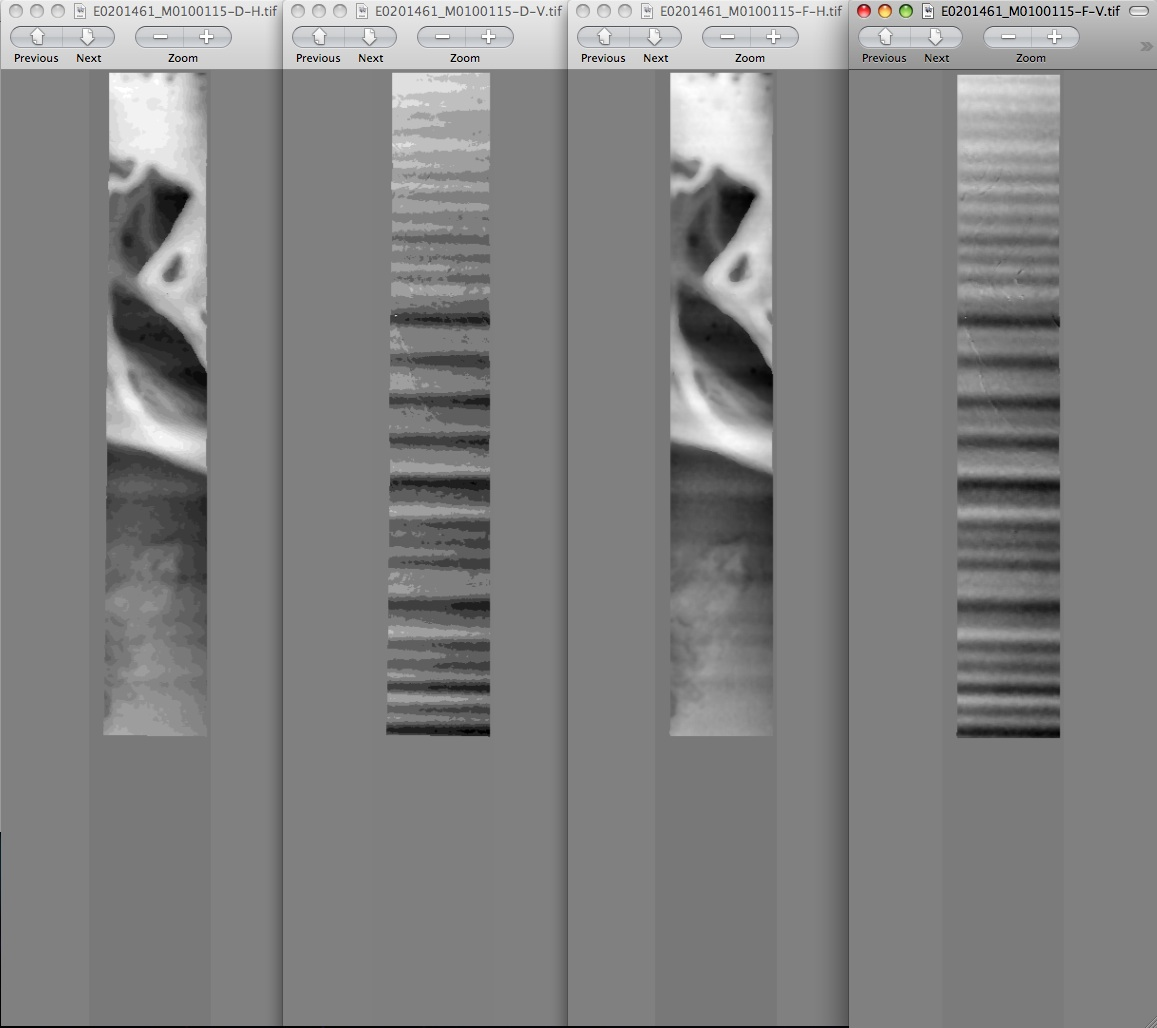
\includegraphics[width=4in]{images/p19-disparity.png}
\end{minipage}
\hfill
\begin{minipage}{2.7in}
\caption[P19 disparity images]{
    \label{p19-disparity}
	Disparity images produced using the \texttt{disparitydebug}
        tool.  The two images on the left are the
        \texttt{E0201461-M0100115-D-H.tif} and
        \texttt{E0201461-M0100115-D-V.tif} files, which are normalized
        horizontal and vertical disparity components produced by the
        disparity map initialization phase.  The two images on the
        right are \texttt{E0201461-M0100115-F-H.tif} and
        \texttt{E0201461-M0100115-F-V.tif}, which are the final
        filtered, sub-pixel-refined disparity maps that are fed into the
        Triangulation phase to build the point cloud image.  Since
        these MOC images were acquired by rolling the spacecraft
        across-track, most of the disparity that represents topography
        is present in the horizontal disparity map.  The vertical
        disparity map shows disparity due to ``wash-boarding,'' which
        is not from topography but from spacecraft movement. Note
        however that the horizontal and vertical disparity images are
        normalized independently.  Although both have the same range
        of gray values from white to black, they represent
        significantly different absolute ranges of disparity.}
\end{minipage}
\end{figure}

\clearpage

\section{Visualizing and Manipulating the Results}
\label{visualising}

When \texttt{stereo} finishes, it will have produced a point cloud
image.  At this point, many kinds of data products can be built from
the \texttt{E0201461-M0100115-PC.tif} point cloud file.

\subsection{Building a 3D Model}

If you wish to see the data in an interactive 3D browser, then you can
generate a 3D object file using the \texttt{point2mesh} command (page
\pageref{point2mesh}). The resulting file is stored in Open Scene
Graph binary format \cite{OSG_website}.  It can be viewed with
\texttt{osgviewer} (the Open Scene Graph Viewer program, distributed
with the binary version of the Stereo Pipeline).  The
\texttt{point2mesh} program takes the point cloud file and the left
normalized image as inputs:

\begin{verbatim}
    ISIS 3> point2mesh E0201461-M0100115-PC.tif E0201461-M0100115-L.tif -l
\end{verbatim}

\noindent
When the \texttt{osgviewer} program starts, you may want to toggle the
lighting with the `L' key, toggle texturing with the 'T' key, and
toggle wireframe mode with the 'W'.  Press '?' to see a variety of
other interactive options.

\begin{figure}[h!]
\begin{minipage}{5in}
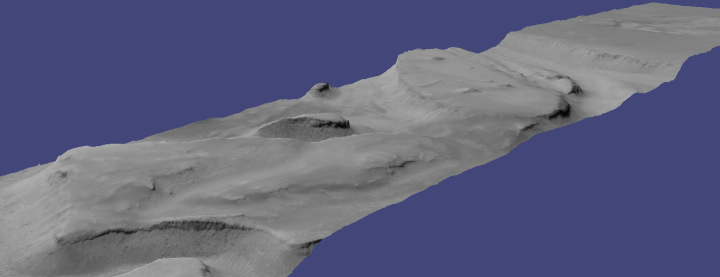
\includegraphics[width=5in]{images/p19-osg.png}
\end{minipage}
\hfill
\begin{minipage}{1.7in}
\caption[P19 in OSG]{
    \label{p19-osg}
	The \texttt{E0201461-M0100115.ive} file displayed in the OSG
        Viewer.  }
\end{minipage}
\end{figure}

\subsection{Building a Digital Elevation Model}

The \texttt{point2dem} program (page \pageref{point2dem}) creates a
Digital Elevation Model (\ac{DEM}) from the point cloud file.

\begin{verbatim}
    ISIS 3> point2dem E0201461-M0100115-PC.tif
\end{verbatim}

\noindent
The resulting TIFF file is map-projected and will contain
georeferencing information stored as GeoTIFF tags. You can specify a
coordinate system (e.g., mercator, sinusoidal) and a reference
spheroid (i.e., calculated for the Moon or Mars).

\begin{verbatim}
    ISIS 3> point2dem -r mars E0201461-M0100115-PC.tif
\end{verbatim}

\noindent
This product is suitable for scientific use, and can be imported into
a variety of GIS platforms.  However, the resulting file,
\texttt{E0201461-M0100115-DEM.tif}, will have 32-bit floating point
pixels, and will not render well in typical image viewers.

The \texttt{point2dem} program can also be used to orthoproject raw
satellite imagery onto the \ac{DEM}. To do this, invoke
\texttt{point2dem} just as before, but add the \texttt{-\/-orthoimage}
option and specify the use of the left image file as the texture file
to use for the projection:

\begin{verbatim}
    ISIS 3> point2dem -r mars --orthoimage E0201461-M0100115-L.tif \
        E0201461-M0100115-PC.tif
\end{verbatim}

\noindent
The \texttt{point2dem} program is also able to accept output
projection options the same way as the tools in GDAL. Well known EPSG,
IAU2000 projections, and custom Proj4 strings can applied with the
target spatial reference set flag, \texttt{-\/-t\_srs}. If the target
spatial reference flag is applied with any of the reference spheroid
options, the reference spheroid option will overwrite the datum
defined in the target spatial reference set. The following examples
produce the same output.

\begin {verbatim}
    ISIS 3> point2dem --t_srs IAU2000:49900 E0201461-M0100115-PC.tif
    ISIS 3> point2dem --t_srs "+proj=longlat +a=3396190 +b=3376200"
        E0201461-M0100115-PC.tif
\end{verbatim}

\noindent
The \texttt{point2dem} program can be used in many different ways.  Be
sure to take your time to explore all of the options.

\begin{figure}
\hfill
\begin{minipage}{3.5in}
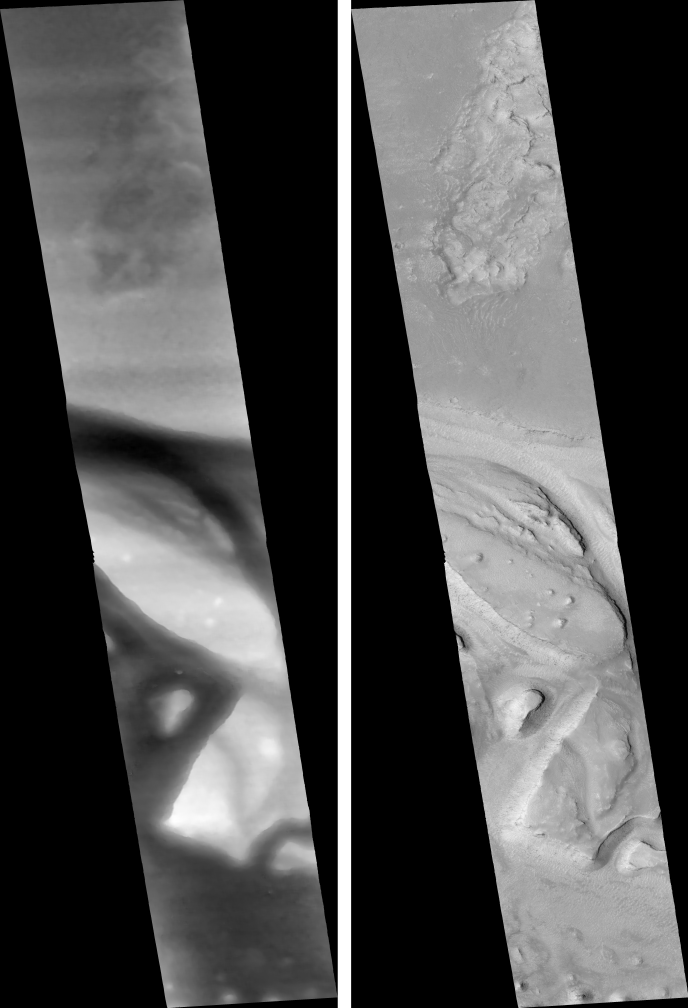
\includegraphics[width=3.5in]{images/p19-norm_ortho.png}
\end{minipage}
\hfill
\begin{minipage}{2in}
\caption[P19 Normalized DEM and Orthophoto]{
    \label{p19-norm_ortho}
	The image on the left is a normalized DEM (generated using the
        \texttt{-n} option), which shows low terrain values as black
        and high terrain values as white.  The image on the right is
        the left input image projected onto the DEM (created using the
        \texttt{-\/-orthoimage} option to \texttt{point2dem}).  }
\end{minipage}
\hfill
\end{figure}

% \begin{figure}
% \begin{center}
% 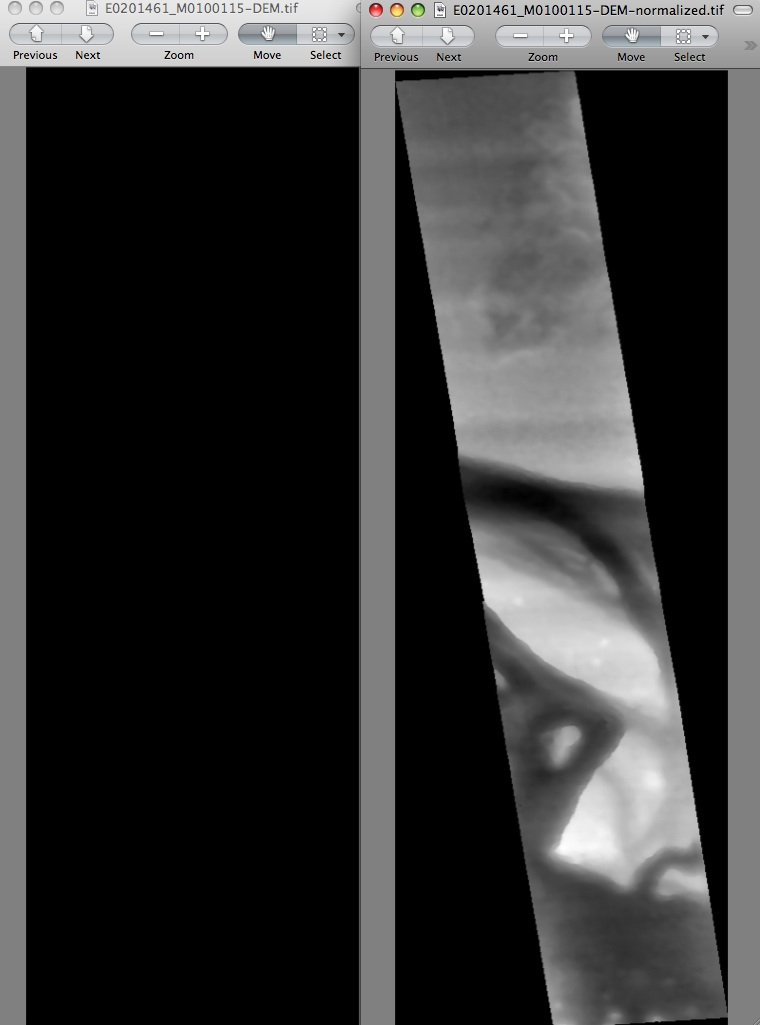
\includegraphics[width=4in]{images/p19-dems.png}
% \caption[P19 dem images]{
%     \label{p19-dems}
%	The non-normalized and normalized DEMs. Note that the
%	non-normalized version contains floating point pixel values
%	and will not open in most image viewing programs which
%	expect integer pixel values between 0 and 255 (which is
%	what the normalized version does for you).
%     }
% \end{center}
% \end{figure}
%
% \begin{figure}
% \begin{center}
% \includegraphics[width=3in]{images/p19-ortho.png}
% \caption[P19 orthophoto]{
%     \label{p19-ortho}
%	The left image orthoprojected onto the DEM.
%     }
% \end{center}
% \end{figure}

\clearpage

\subsection{Creating DEMs relative to the Geoid/Areoid}

The DEMs generated using \texttt{point2dem} are in reference to a datum
ellipsoid. If desired, the \texttt{dem\_geoid} program can be used to
convert this DEM to be relative to a geoid/areoid on Earth/Mars
respectively.

\subsection{Converting to the LAS Format}

If it is desired to use the generated point cloud in contexts outside
ASP, it can be converted to the LAS file format, which is a public file
format for the interchange of 3-dimensional point cloud data. The tool
\texttt{point2las} can be used for that purpose (section \ref{point2las}).

\subsection{Generating Color Hillshade Maps}

Once you have generated a \ac{DEM} file, you can use the Vision Workbench's
\texttt{colormap} and \texttt{hillshade} tools to create colorized
and/or shaded relief images.

To create a colorized version of the \ac{DEM}, you need only specify
the \ac{DEM} file to use. The colormap is applied to the full range of
the DEM, which is computed automatically.  Alternatively you can
specific your own min and max range for the color map.

\begin{verbatim}
    ISIS 3> colormap E0201461-M0100115-DEM.tif -o hrad-colorized.tif
\end{verbatim}

To create a hillshade of the \ac{DEM}, specify the \ac{DEM} file to
use. You can control the azimuth and elevation of the light source
using the \texttt{-a} and \texttt{-e} options.

\begin{verbatim}
    ISIS 3> hillshade E0201461-M0100115-DEM.tif -o hrad-shaded.tif -e 25
\end{verbatim}

To create a colorized version of the shaded relief file, specify
the \ac{DEM} and the shaded relief file that should be used:

\begin{verbatim}
    ISIS 3> colormap E0201461-M0100115-DEM.tif -s hrad-shaded.tif -o hrad-color-shaded.tif
\end{verbatim}

\begin{figure}[b!]
\begin{center}
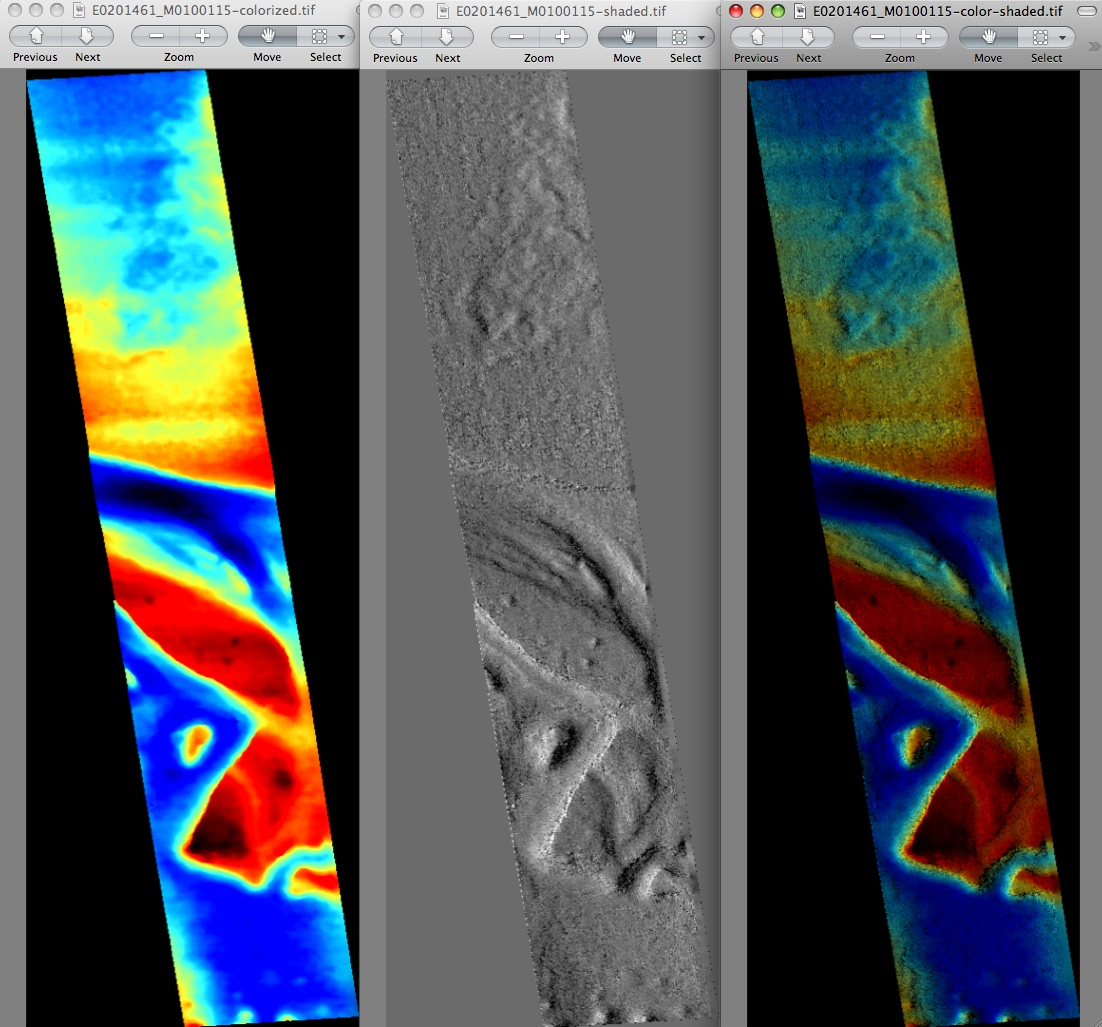
\includegraphics[width=4.7in]{images/p19-colorized-shaded.png}
\caption[Hrad colorized and shaded relief]{
    \label{hrad-color}
	The colorized DEM, the shaded relief image, and the colorized hillshade.
    }
\end{center}
\end{figure}

\clearpage

\subsection{Building Overlays for Moon and Mars mode in Google Earth}

The final program in the Stereo Pipeline package that this tutorial
will address is \texttt{image2qtree}.  This tool was designed to
create tiled, multi-resolution overlays for Google Earth.  In addition
to generating image tiles, it produces a metadata tree in KML format
that can be loaded from your local hard drive or streamed from a
remote server over the Internet.

The \texttt{image2qtree} program can only be used on 8-bit image files
with georeferencing information (e.g. grayscale or RGB geotiff
images). In this example, it can be used to process \\
\texttt{E0201461-M0100115-DEM-normalized.tif},
\texttt{E0201461-M0100115-DRG.tif} \texttt{hrad-shaded.tif}, \\
\texttt{hrad-colorized.tif}, and \texttt{hrad-shaded-colorized.tif}

\begin{verbatim}
    ISIS 3> image2qtree hrad-shaded-colorized.tif -m kml --draw-order 100
\end{verbatim}

\begin{figure}[b!]
\begin{center}
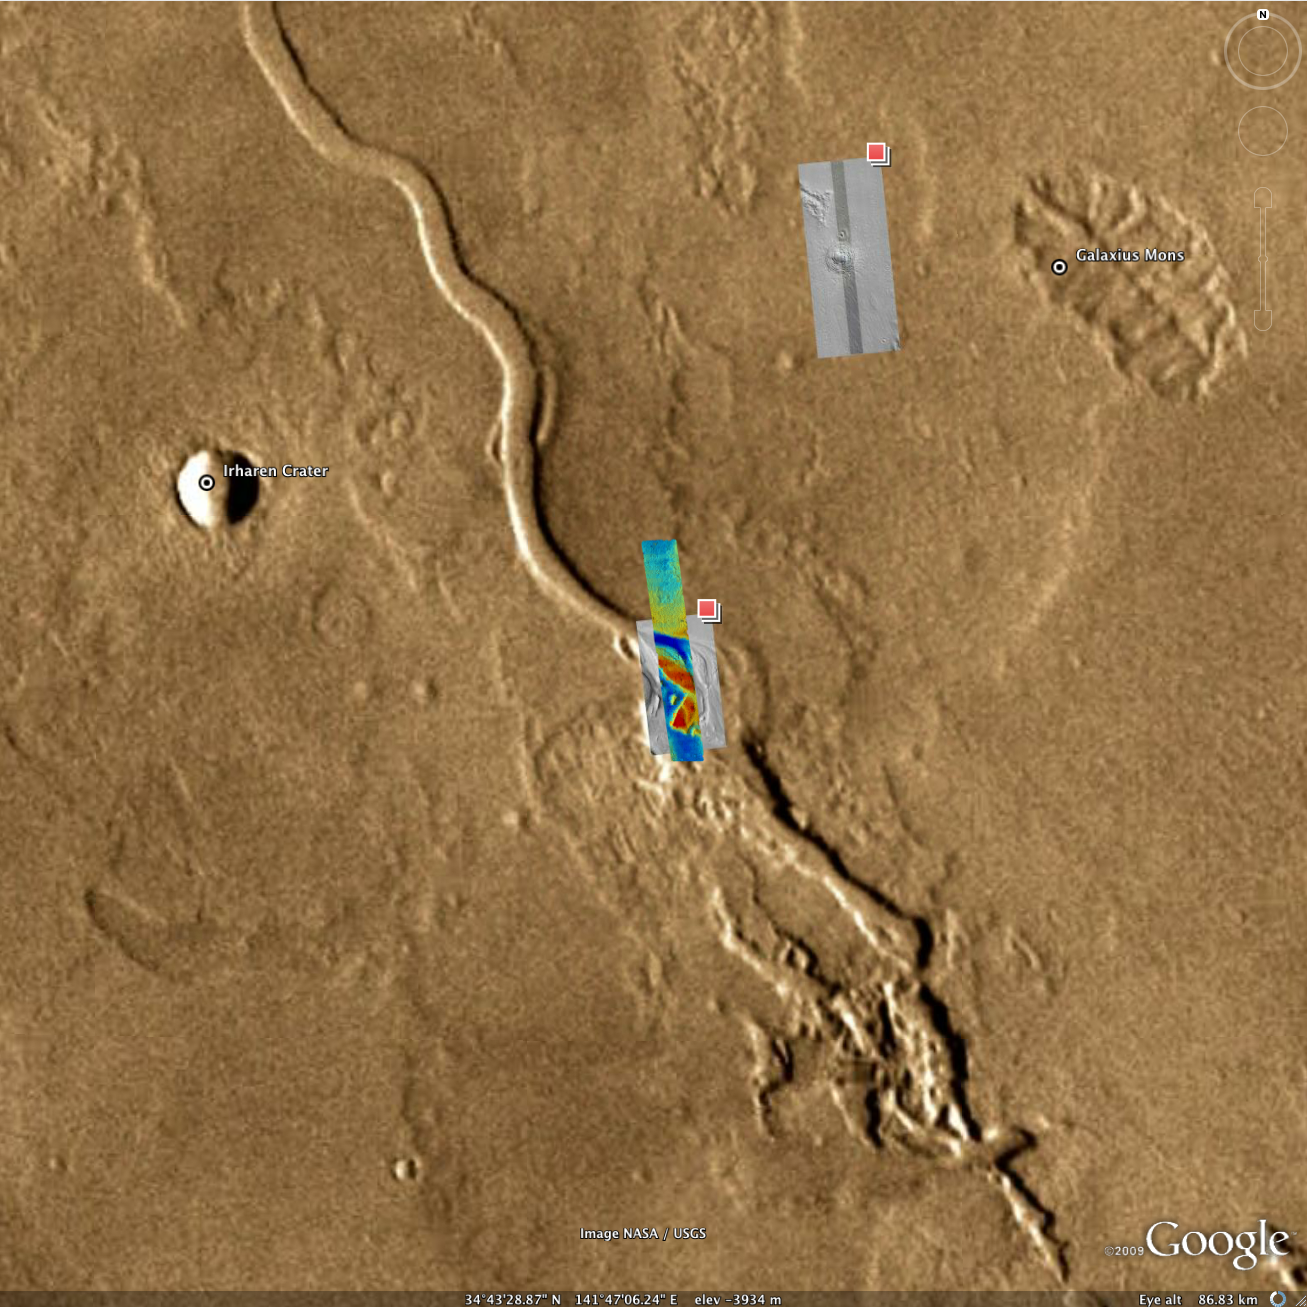
\includegraphics[width=6in]{images/p19-googlemars.png}
\caption[Hrad shaded colorized DEM as a KML overlay] {
    \label{hrad-kml}
        The colorized hillshade DEM as a KML overlay.  }
\end{center}
\end{figure}
